%%%%%%%%%%%%%%%%%%%%%%%%%%%%%%%%%%%%%%
%%%%%%%%%%%%%%%%%%%%%%%%%%%%%%%%%%%%%%
% Do not edit the TeX file your work
% will be overwritten.  Edit the RnW
% file instead.
%%%%%%%%%%%%%%%%%%%%%%%%%%%%%%%%%%%%%%
%%%%%%%%%%%%%%%%%%%%%%%%%%%%%%%%%%%%%%












% \def\ARMTable{
% \begin{table}[h]
% <<arm_model_table, cache=cache_arm, results='asis'>>=
% source("R_scripts/ARM/model_table.R", echo=knitr_debug, print.eval=TRUE)
% @
% \caption{Models from \cite{gelman:2006:arm}\tablabel{arm_models}}
% \end{table}
% }




\def\OttoGraphZero{
%

\begin{knitrout}
\definecolor{shadecolor}{rgb}{0.969, 0.969, 0.969}\color{fgcolor}\begin{figure}[!h]

{\centering 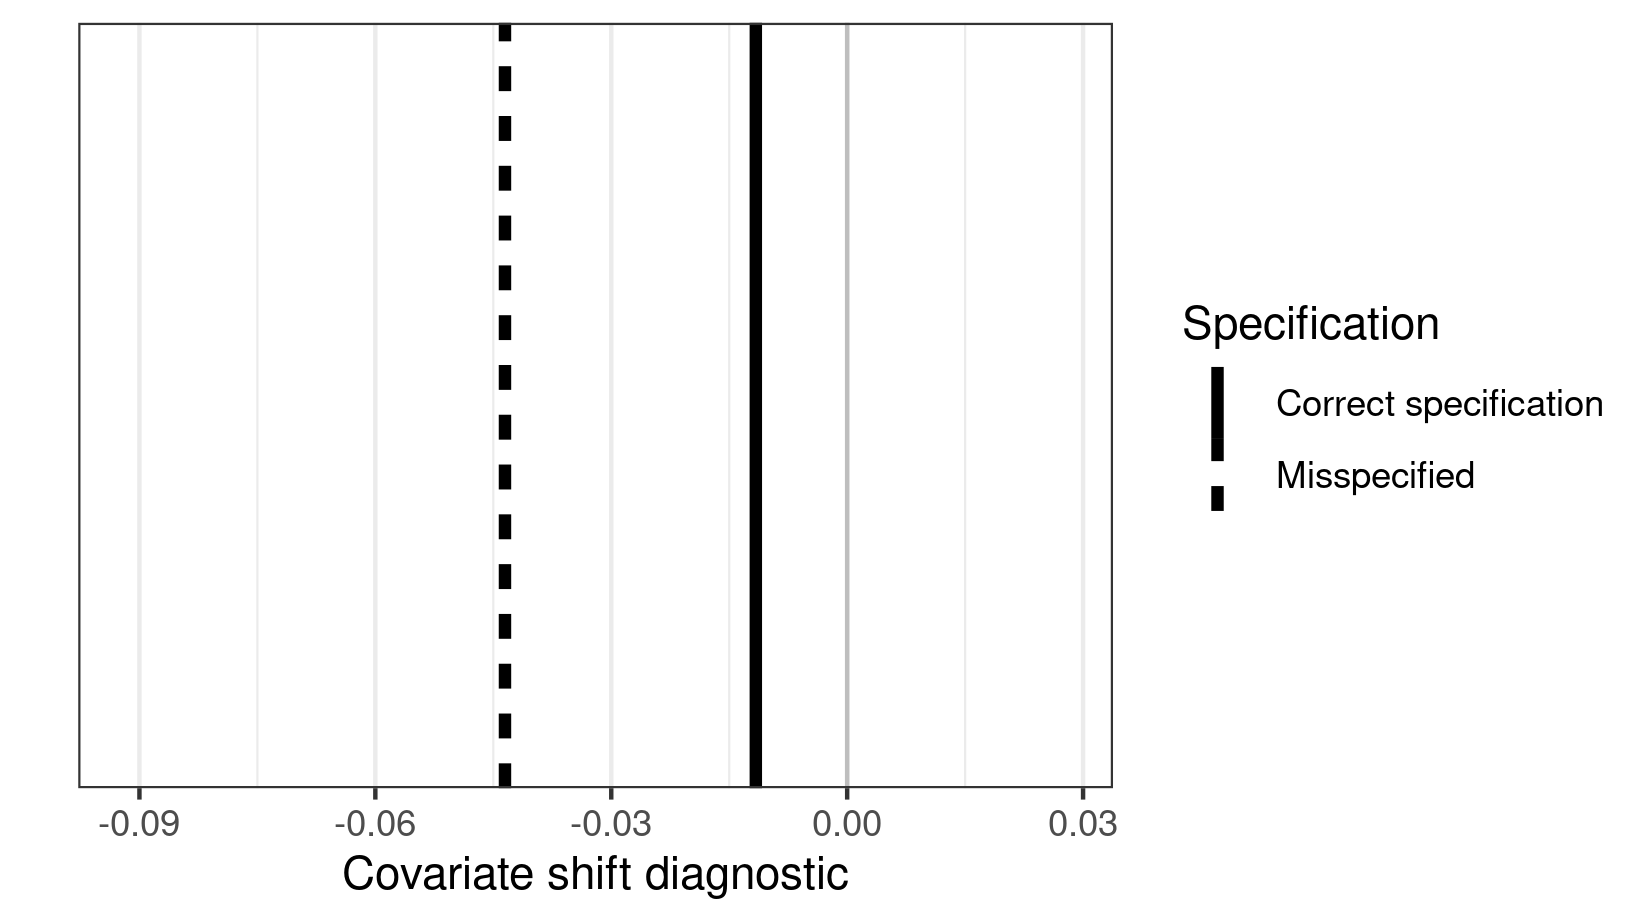
\includegraphics[width=0.98\linewidth,height=0.549\linewidth]{figure/ottograph0-1} 

}

\caption[A covariate shift diagnostic]{A covariate shift diagnostic}\label{fig:ottograph0}
\end{figure}

\end{knitrout}
}

\def\OttoGraphOne{
%

\begin{knitrout}
\definecolor{shadecolor}{rgb}{0.969, 0.969, 0.969}\color{fgcolor}\begin{figure}[!h]

{\centering 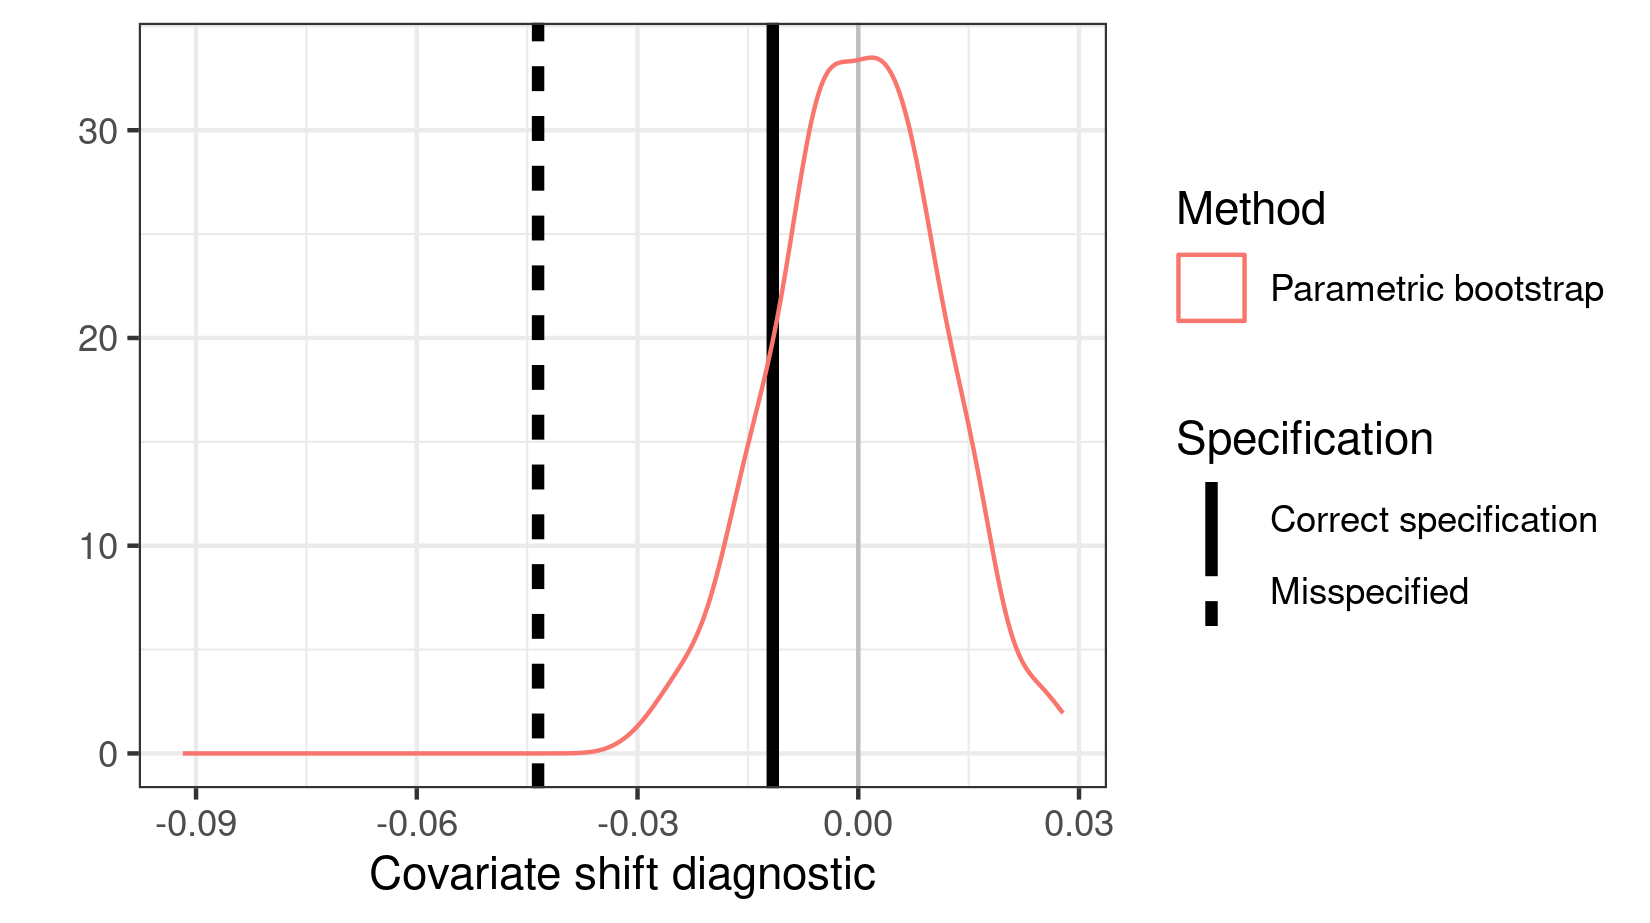
\includegraphics[width=0.98\linewidth,height=0.549\linewidth]{figure/ottograph1-1} 

}

\caption[A covariate shift diagnostic]{A covariate shift diagnostic}\label{fig:ottograph1}
\end{figure}

\end{knitrout}
}


\def\OttoGraphTwo{
%

\begin{knitrout}
\definecolor{shadecolor}{rgb}{0.969, 0.969, 0.969}\color{fgcolor}\begin{figure}[!h]

{\centering 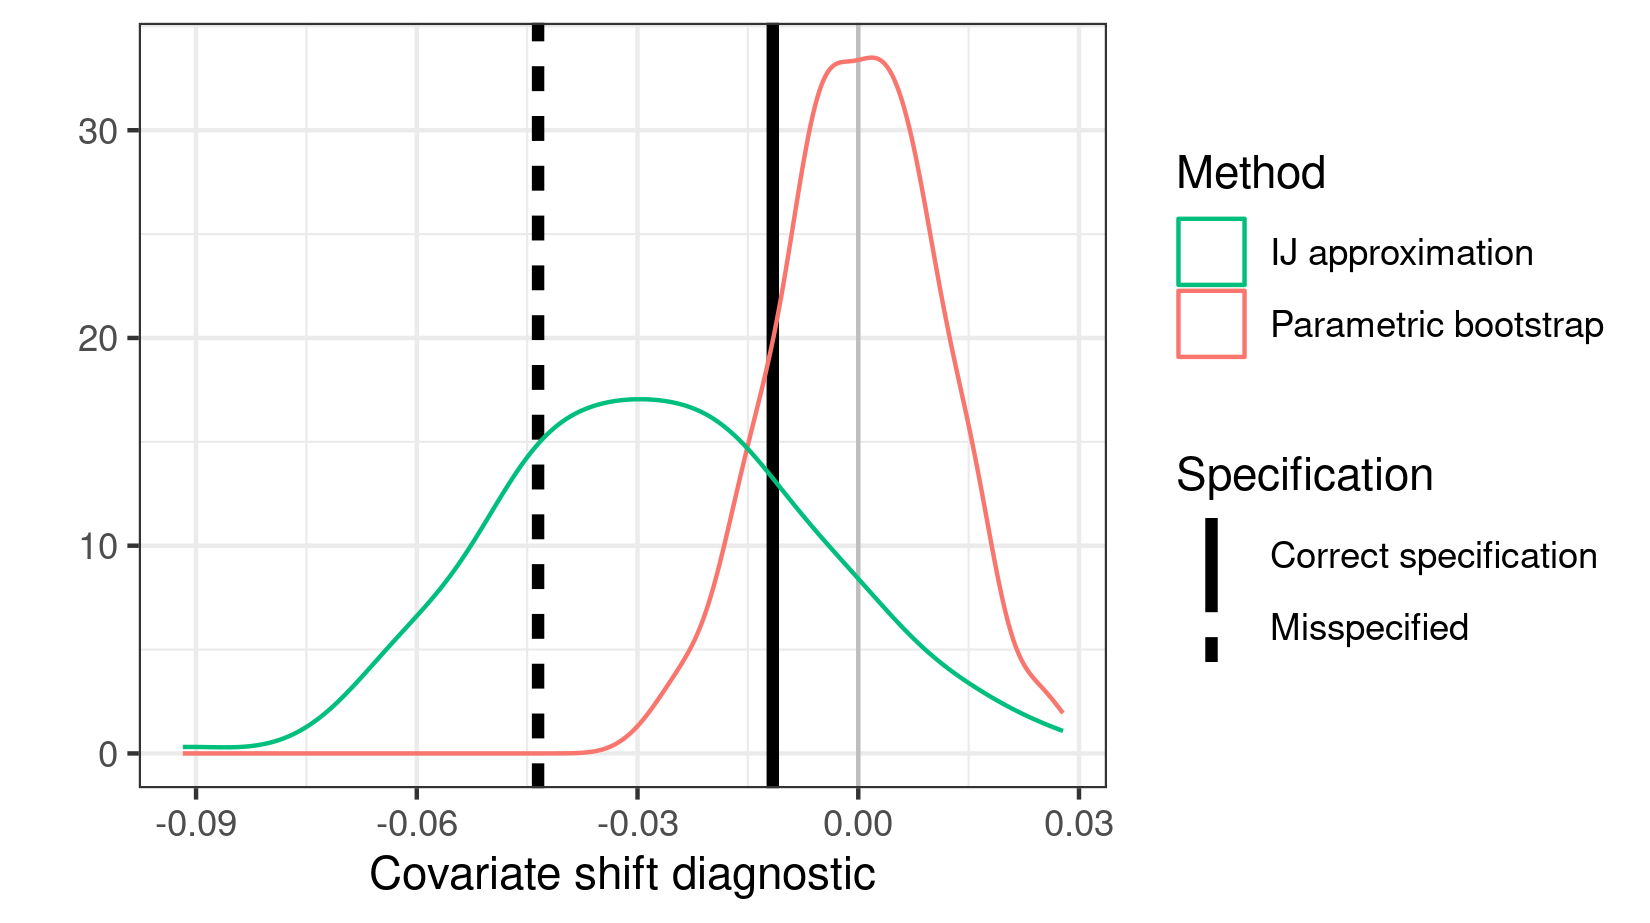
\includegraphics[width=0.98\linewidth,height=0.549\linewidth]{figure/ottograph2-1} 

}

\caption[A covariate shift diagnostic]{A covariate shift diagnostic}\label{fig:ottograph2}
\end{figure}

\end{knitrout}
}


\def\OttoGraphThree{
%

\begin{knitrout}
\definecolor{shadecolor}{rgb}{0.969, 0.969, 0.969}\color{fgcolor}\begin{figure}[!h]

{\centering 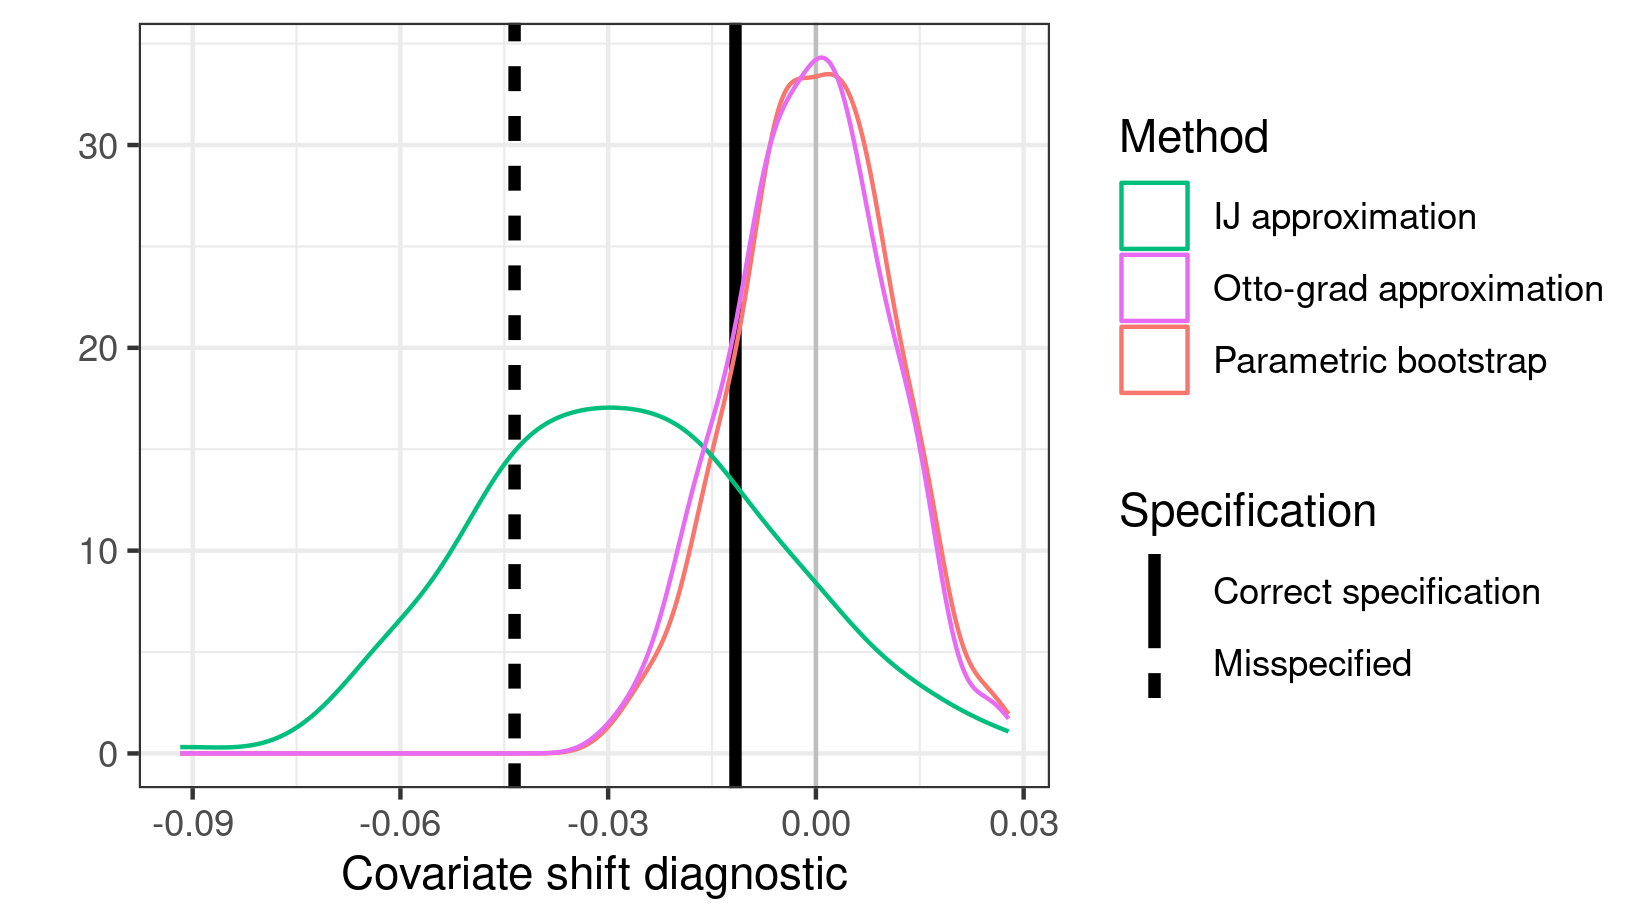
\includegraphics[width=0.98\linewidth,height=0.549\linewidth]{figure/ottograph3-1} 

}

\caption[A covariate shift diagnostic]{A covariate shift diagnostic}\label{fig:ottograph3}
\end{figure}

\end{knitrout}
}



